\section{Evaluation Metrics}
The evaluation metrics used to measure the performance of the Biometric Systems in the 3 experimental scenarios are liste below.

\begin{itemize}

    \item \textbf{False Acceptance Rate (FAR)}:  
    Percentage of impostor samples incorrectly accepted by the system.  
    \[
    \text{FAR} = \frac{\text{Number of False Acceptances}}{\text{Total Number of Impostor Attempts}} \times 100
    \]
    Lower FAR values indicate a more secure system while a higher FAR signifies a higher risk of impostor acceptance.
    
    \item \textbf{False Rejection Rate (FRR)}:  
    Percentage of genuine samples incorrectly rejected by the system.  
    \[
    \text{FRR} = \frac{\text{Number of False Rejections}}{\text{Total Number of Genuine Attempts}} \times 100
    \]
    Lower FRR values indicate a more reliable system while a higher FRR signifies a higher risk of genuine rejection.

    \item \textbf{Equal Error Rate (EER)}:  
    The point where the FAR and FRR are equal, providing a single measure of system performance.  
    A lower EER signifies a more balanced system.

    \item \textbf{Receiver Operating Characteristic (ROC) Curve}:  
    Curve plotted on a Cartesian plane where the axes are Genuine Acceptance Rate and False Acceptance Rate. It represents the probability of correctly identifying a subject as the FAR varies.

    \item \textbf{Detection Error Tradeoff (DET) Curve}:  
    A variation of the ROC curve that plots the FRR against the FAR on a logarithmic scale, providing insight into trade-offs between errors.

    \item \textbf{Cumulative Match Characteristic (CMC) Curve}:  
    Represents the probability of correct identification as a function of rank in a closed-set scenario. Higher Rank-1 and rapid convergence to 1.0 indicate strong identification performance.

    \item \textbf{Confusion Matrix}:  
    The confusion matrix is a tool used to evaluate the performance of a classification model. It consists of a table where the columns are Predicted Negative and Predicted Positive, while the rows are Real Negative and Real Positive, comparing the model's predictions with the actual classes of the dataset. Below is a generic representation of a confusion matrix:
    \[
    \begin{array}{c|c|c}
          & \text{PN} & \text{PP} \\ \hline
        \text{RN} & \text{TN} & \text{FP} \\ 
        \text{RP} & \text{FN} & \text{TP} \\
    \end{array}
    \]
  
    \begin{itemize}
        \item \textbf{FP (False Positive)}:  
        The model incorrectly predicted that an instance belongs to the positive class when it actually belongs to the negative class (false alarm).
        
        \item \textbf{FN (False Negative)}:  
        The model incorrectly predicted that an instance belongs to the negative class when it actually belongs to the positive class (missed detection).
        
        \item \textbf{TN (True Negative)}:  
        The model correctly predicted that an instance belongs to the negative class.
        
        \item \textbf{TP (True Positive)}:  
        The model correctly predicted that an instance belongs to the positive class.
    \end{itemize}

    \item \textbf{Open-set (Watchlist) Receiver Operating Characteristic (ROC)}: Depicts DIR against FAR and is useful for finding the optimal threshold, balancing the maximization of DIR and the minimization of FAR. A compromise is necessary as both measures depend on the threshold, but in opposite directions:
    \begin{itemize}
        \item If we raise the threshold, FAR decreases, but DIR also decreases.
        \item If we lower the threshold, DIR increases, but FAR also increases.
    \end{itemize}

\end{itemize}

\section{Results}
The results of the evaluation metrics for the Biometric Systems in the 3 experimental scenarios are presented below with comments on the performance of the systems.

\subsection{Identification with a Closed Set}

The biometric system's performance for closed-set identification was evaluated using the Cumulative Match Characteristic (CMC) curve, which measures the probability of correct identification at various ranks.

\begin{figure}[!ht]
    \centering
    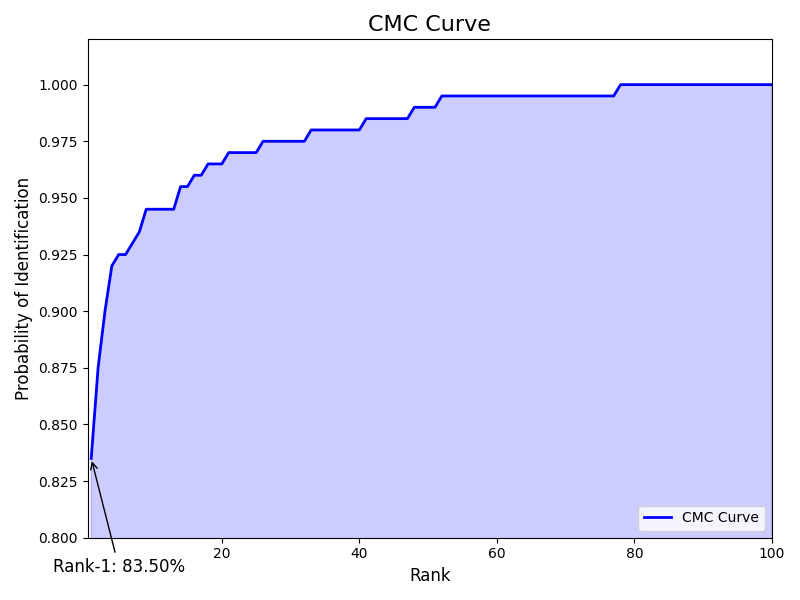
\includegraphics[width=\columnwidth]{./images/plots/id-close/cmc_curve.png}
    \caption{CMC Curve demonstrating the probability of identification across ranks for closed-set identification.}
    \label{fig:cmc_curve}
\end{figure}

\textbf{CMC Curve}: The CMC curve indicates that the system achieves a Rank-1 identification rate of 83.50\%, highlighting its ability to correctly identify subjects in the top rank most of the time. The curve rapidly approaches a probability of 1.0 as the rank increases.

\subsection{Identification with an Open Set}

The biometric system's performance for open-set identification was evaluated using the Watchlist Receiver Operating Characteristic (ROC) curve, plotting the Detection and Identification Rate (DIR) against the False Alarm Rate (FAR).

\begin{figure}[!ht]
    \centering
    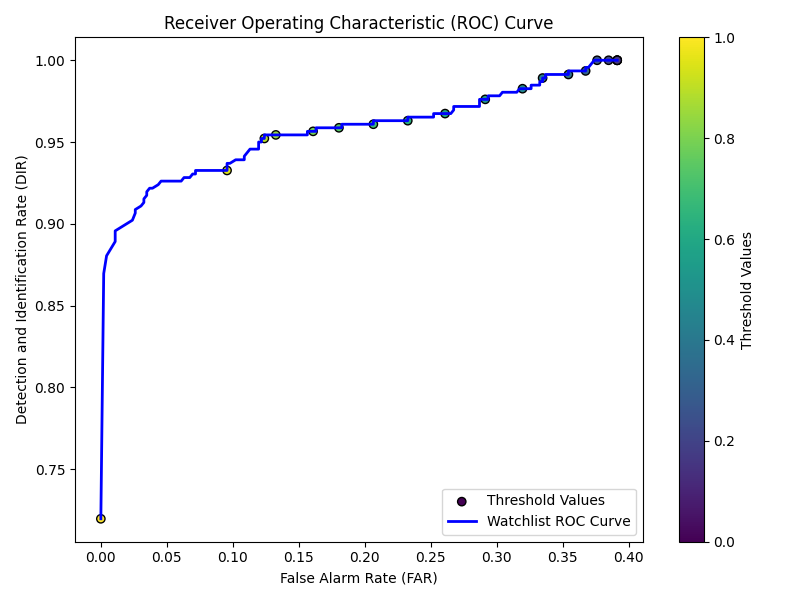
\includegraphics[width=\columnwidth]{./images/plots/id-open/watchlist_roc_curve.png}
    \caption{Watchlist ROC Curve demonstrating the DIR vs. FAR for open-set identification.}
    \label{fig:watchlist_roc_curve}
\end{figure}

\textbf{Watchlist ROC Curve}: The ROC curve demonstrates the system's effectiveness in maintaining a high Detection and Identification Rate (DIR) while minimizing the False Alarm Rate (FAR). The curve achieves strong performance, as evidenced by a consistent increase in DIR with lower FAR values. Threshold markers along the curve provide insights into the system's operating characteristics and trade-offs between detection and false alarms. 

\subsection{Verification}

The biometric verification system was evaluated using False Acceptance Rate (FAR), False Rejection Rate (FRR), Equal Error Rate (EER), Receiver Operating Characteristic (ROC) and Detection Error Tradeoff (DET) curves, and a Confusion Matrix to assess the system's performance.

\begin{figure}[!ht]
    \centering
    \begin{subfigure}[t]{0.48\columnwidth}
        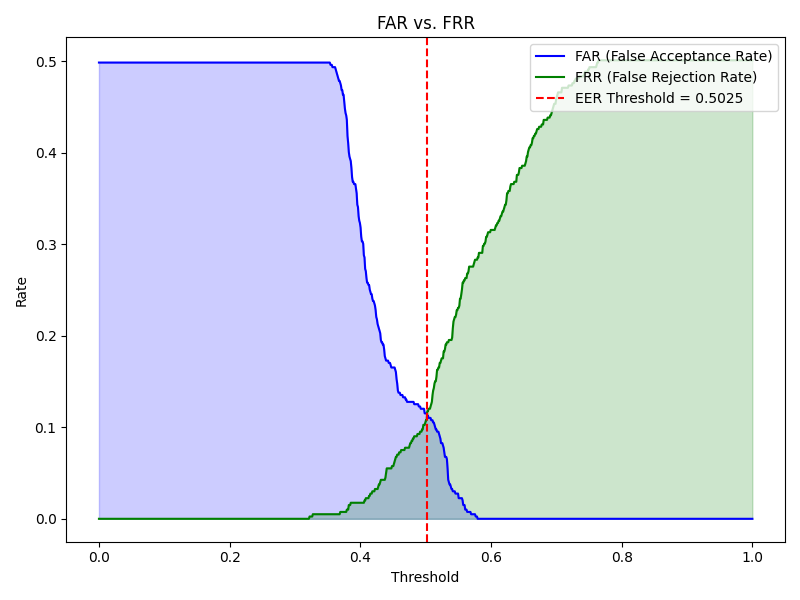
\includegraphics[width=\textwidth]{./images/plots/ver/far_vs_frr.png}
        \caption{FAR vs. FRR}
        \label{fig:far_vs_frr}
    \end{subfigure}
    \hfill
    \begin{subfigure}[t]{0.48\columnwidth}
        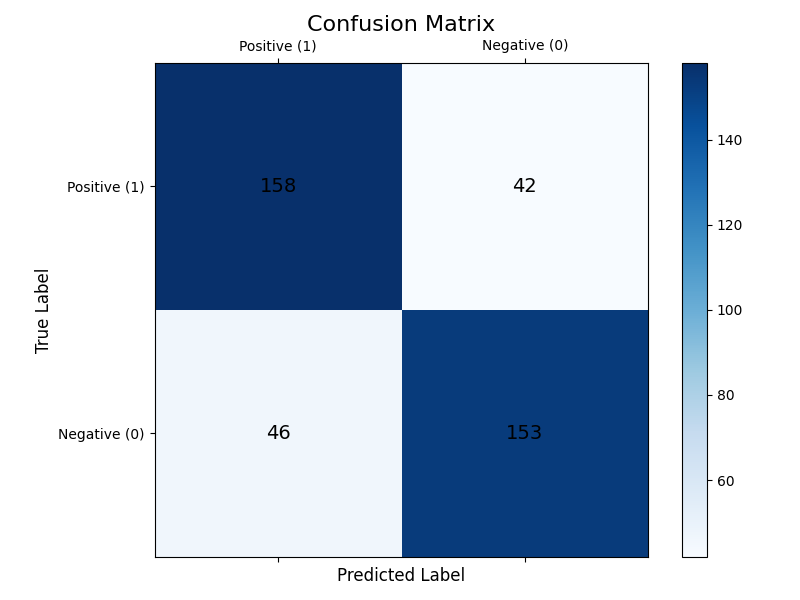
\includegraphics[width=\textwidth]{./images/plots/ver/confusion_matrix.png}
        \caption{Confusion Matrix}
        \label{fig:confusion_matrix}
    \end{subfigure}
\end{figure}

\textbf{FAR vs. FRR Analysis}: The FAR and FRR curves intersect at a threshold of 0.5025, yielding an EER of 0.5025. This indicates a balanced trade-off between the acceptance of impostors and rejection of genuine users.

\textbf{Confusion Matrix}: The system achieved a good balance between true positives (158) and true negatives (153) while maintaining acceptable rates of false positives (42) and false negatives (46).

\begin{figure}[!ht]
    \centering
    \begin{subfigure}[t]{0.48\columnwidth}
        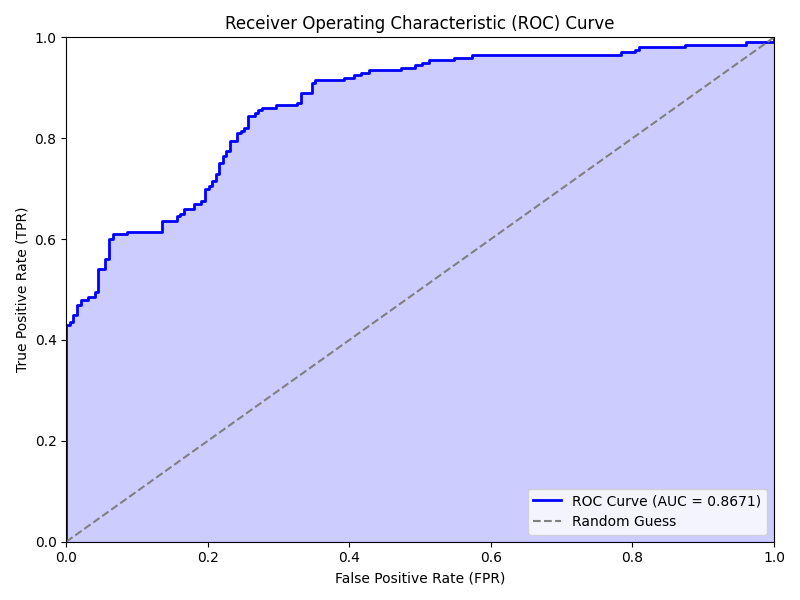
\includegraphics[width=\textwidth]{./images/plots/ver/roc_curve.png}
        \caption{ROC Curve}
        \label{fig:roc_curve}
    \end{subfigure}
    \hfill
    \begin{subfigure}[t]{0.48\columnwidth}
        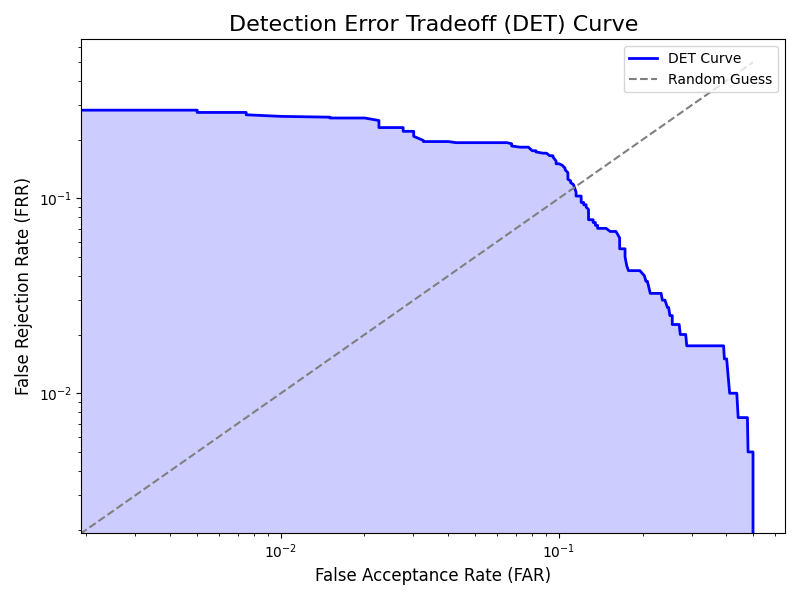
\includegraphics[width=\textwidth]{./images/plots/ver/det_curve.png}
        \caption{DET Curve}
        \label{fig:det_curve}
    \end{subfigure}
\end{figure}

\textbf{ROC Curve}: With an Area Under the Curve (AUC) of 0.8671, the ROC curve demonstrates strong discriminatory power between genuine and impostor samples.

\textbf{Detection Error Tradeoff (DET) Curve}: The DET curve highlights the system's error rates over a range of operating conditions. The downward trend reflects the system's ability to minimize errors as the threshold is optimized.